\documentclass{article}
\usepackage[utf8]{inputenc}
\usepackage[T2A]{fontenc}
\usepackage[russian]{babel}
\usepackage{amsmath}
\usepackage{graphicx}

\begin{document}

\title{Практика 4}
\author{Ращупкин Е, Боков Е, Мишунин Н}
\maketitle

\section{Задача 1}
Автор Author направляет статью SendPaper редактору журнала Edition. Редактор передает статью на рецензирование Review нескольким рецензентам Reviewer. Затем редактор возвращает отзывы рецензентов автору в том же варианте использования SendPaper.

\begin{itemize}
    \item Добавьте возможность автору вместе с корректором ProofReader подготовить статью  к публикации PrepareForPublishing.
    \item Доработайте модель, указав, что подготовка статьи к публикации выполняется, только если она была одобрена редактором в варианте использования SendPaper.
\end{itemize}

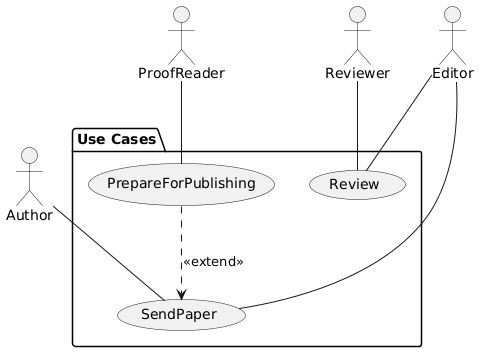
\includegraphics[width=\textwidth]{1.png}

\section{Задача 2}
Распознавателю текста OCRModule от модуля морфологии нужна возможность определить, принадлежит ли слово языку, и функция приведения слова к заданной форме, в частности, восстановления начальной формы. Также нужна функция получения грамматического значения конкретного слова.

\begin{itemize}
    \item Постройте модель системы.
    \item Добавьте функцию вывода слов, похожих на введенное, если его нет в словаре языка. Каким образом данная возможность системы связана с другими функциями?
    \item Укажите в модели, что все перечисленные задачи подразумевают выполнение поиска слова (или его основы) в словаре.
    \item Некоторые языки могут не поддерживаться системой. Перед выполнением любой функции модули морфологии нужно проверить, поддержан ли язык. Отобразите это в модели.
\end{itemize}

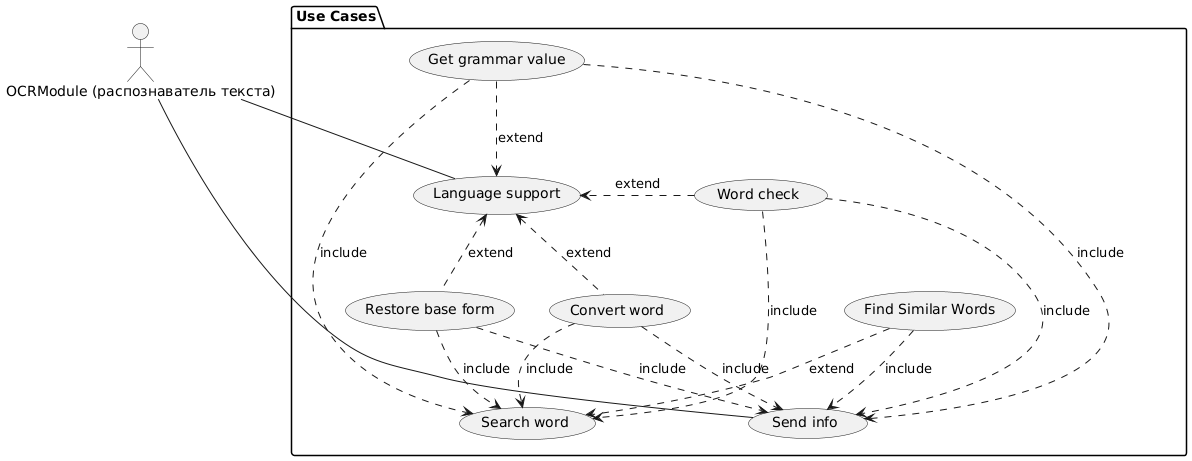
\includegraphics[width=\textwidth]{2.png}

\section{Задача 3}
Ответственное лицо ResponsiblePerson может прикрепить документ AttachIssue к обсуждаемому вопросу, выступая в роли автора author, и к постановлению AttachResolution, выступая в роли председателя chairman.

\begin{itemize}
    \item Покажите в модели, что прикрепление документа выполняется согласно общему сценарию прикрепления AttachDocument, реализуемому в частном случае прикрепления к вопросу или прикрепления к постановлению. Ответственное лицо участвует в сценарии прикрепления в роли пользователя user, объединяющей роли автора и председателя.
    \item Добавьте в модель оператора Operator, который является ответственным лицом с возможностью удаления документов DeleteDocument.
    \item Доработайте модель, указав, что при прикреплении документа рассылается оповещение SendAnnouncement. Несколько операторов могут выступать в роли контролеров controller.
    \item Каким образом можно указать, что прикрепление документа возможно только к вопросу или к постановлению? Ответ поясните.
\end{itemize}

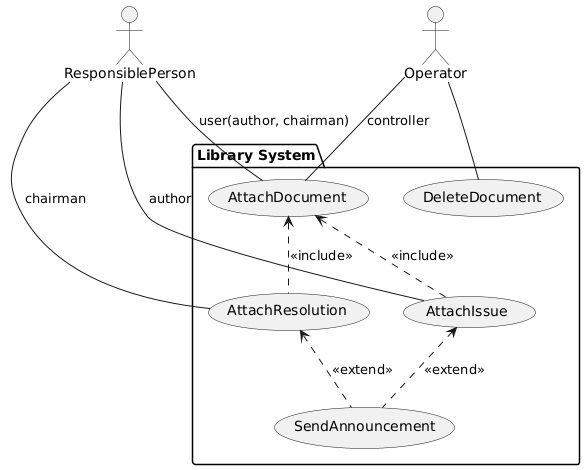
\includegraphics[width=\textwidth]{3.png}

\section{Задача 4}
Пользователь User настраивает подключаемые модули аудиоплеера AudioPlayer в рамках варианта использования ConfigurePlugins.

\begin{itemize}
    \item Добавьте к варианту использования ConfigurePlugins возможность выбора определенного плагина для настройки SelectPlugin и возможность настройки конкретного плагина ChangeSettings. 
    \item Добавьте в модель возможность обновить плагины UpdatePlugins с внешнего сервера плагинов PluginsServer.
    \item Помимо обычного пользователя в системах обычно есть привилегированный пользователь SuperUser, который имеет права на изменение конфигурации системы. В системе аудиоплеера такой пользователь может обновить плагины UpdatePluginsList. Обновление включает в себя удаление DeletePlugins, установку InstallPlugins и просмотр списка доступных на сервере плагинов CheckPluginsList.
\end{itemize}

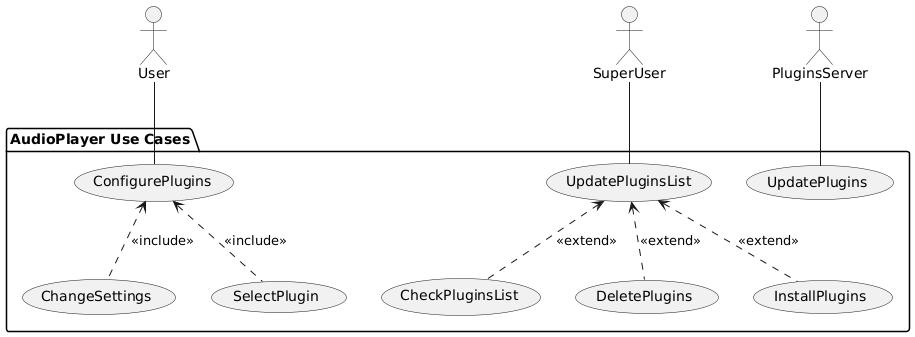
\includegraphics[width=\textwidth]{4.png}

\section{Задача 5}
Рассмотрим электронную библиотеку научных работ.

\begin{itemize}
    \item Поясните, каким образом используется электронная библиотека. Перечислите актеров и варианты использования.
    \item Укажите, что аналитик Analyst принимает участие в индексировании статей, выполняемом в процессе их загрузки бизнес-партнером Content partner.
    \item Предоставьте возможность исследователю Reseacher использовать расширенный поиск AdvancedSearch, который позволяет указать другие параметры поиска в FindPapers.
    \item Укажите, что все варианты использования преследуют цели пользователей (user goal) системы.
\end{itemize}

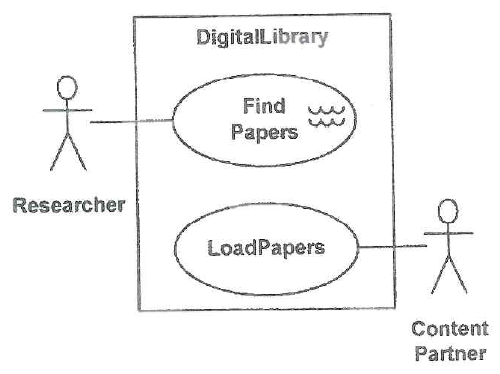
\includegraphics[width=\textwidth]{task5.png}
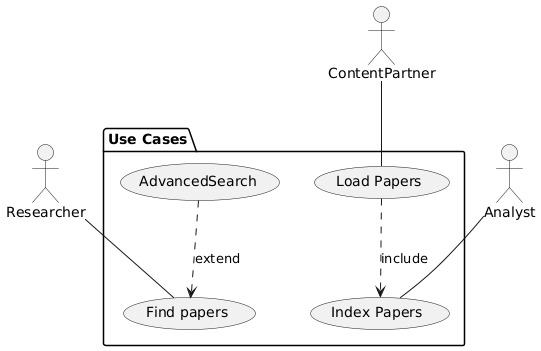
\includegraphics[width=\textwidth]{5.png}

\section{Задача 6}
Клиент Client выполняет операции над своими счетами в банке Bank, используя банкомат ATM в рамках абстрактного варианта использования PerformOperation, который включает информирование об услугах в варианте использования InformAboutServices. Для выполнения операций ATM обращается к платежной системе PaymentSystem.

\begin{itemize}
    \item Перечислите основных и вспомогательных актеров системы ATM. Какие из них взаимодействуют с системой в варианте использования PerformOperation?
    \item Отразите в модели вариантов использования, что клиенты могут только выполнять операции по получению наличных, в то время как клиенты Bank Customers банка, владеющего банкоматом, могут также оплачивать услуги из списка, предоставляемого банком Bank. При этом сценарии при оплате услуг и получения наличных отличаются между собой, не следуют общему сценарию выполнения операций.
    \item Добавьте возможность получения наличных, как в валюте счета, так и в другой валюте. При этом в обоих случаях банкомат запрашивает у клиента Client подтверждение на списание средств в валюте счета по курсу банка Bank.
\end{itemize}

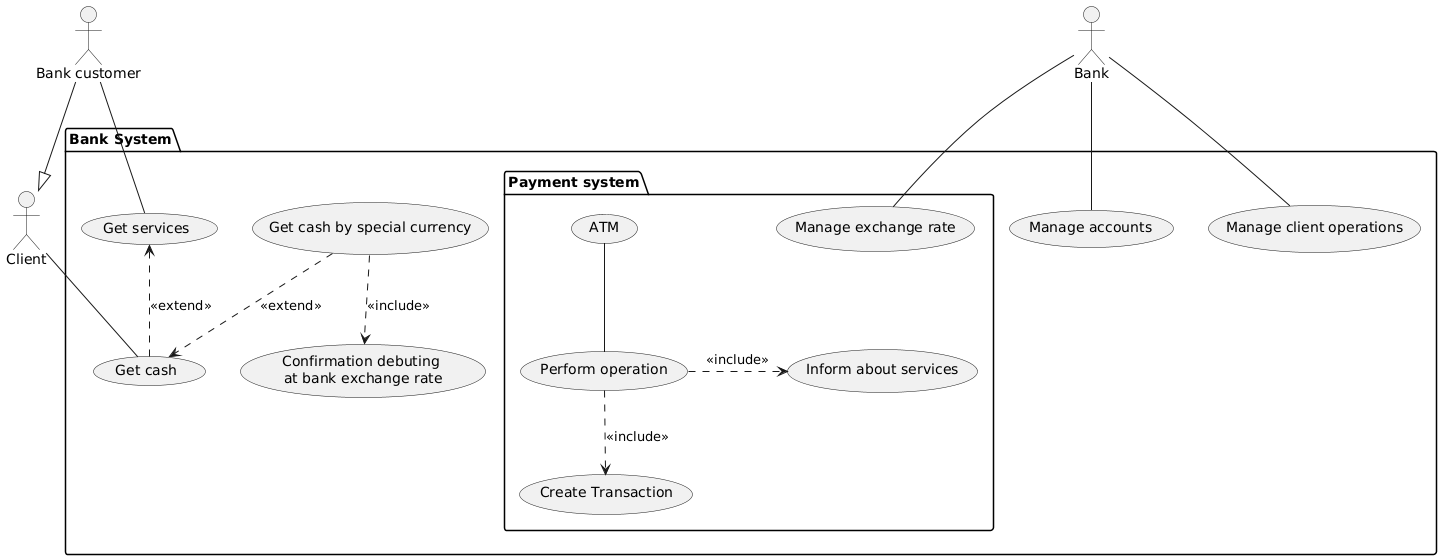
\includegraphics[width=\textwidth]{6.png}

\section{Задача 7}
Во время подготовки данных для морфологического модуля актер лингвист Linguist взаимодействует с системой подготовки данных MorphoDB посредством абстрактного варианта использования изменения данных ModifyData. Кроме того, для проверки целостности модифицируемых данных лингвисты могут компилировать данные Compile. Компиляция также включает в себя экспорт данных ExportData в формат, понимаемый компилятором. Каждую ночь сервер сборки приложения BuildServer компилирует данные посредством варианта использованию Compile.

\begin{itemize}
    \item Добавьте в систему программиста Programmer, которому доступны те же возможности, что и лингвисту. Кроме того, он может экспортировать данные ExportData для отладки подсистемы компиляции данных.
    \item Укажите, что для повторного использования словаря, который хранится на сервере данных морфологии, модуль семантики Semantics может взаимодействовать с системой подготовки данных морфологии в варианте использования ExportWordList.
    \item Добавьте функции изменения данных: добавление, удаление, изменение слова.
    \item Добавьте в модель возможность при изменении данных в некоторых случаях проверять целостность данных перед сохранением в систему.
    \item Будет ли проверяться целостность данных при удалении слова? Ответ поясните.
    \item Проведите количественную оценку диаграммы.
\end{itemize}

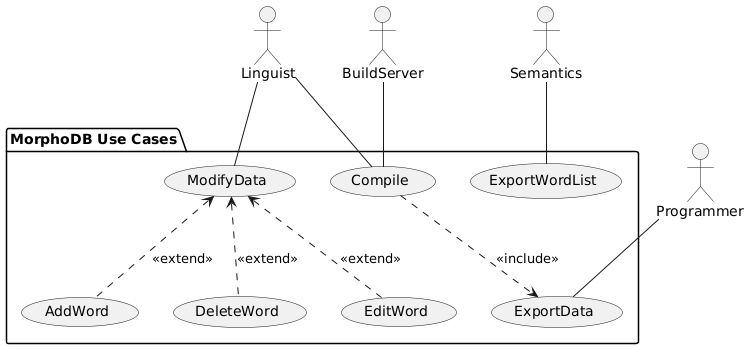
\includegraphics[width=\textwidth]{7.png}

\begin{itemize}
    \item 7 прецедентов (вариантов использования), каждый из которых оценивается в 2 балла.
    \item 5 ассоциаций, каждая из которых оценивается в 1 балл.
    \item 5 остальных связей, каждая из которых оценивается в 1 балл.
\end{itemize}


\[
7 \, (\text{прецедентов}) \times 2 = 14
\]
\[
5 \, (\text{ассоциаций}) \times 1 = 5
\]
\[
5 \, (\text{остальных связей}) \times 1 = 5
\]

\[
S = \frac{(14 + 5 + 5)}{(1 + 11 + \sqrt{1 + 1})}
\]

\[
S \approx 1.79
\]

Таким образом, коэффициент сложности диаграммы равен \( S \approx 1.79 \).

\end{document}
